\begin{center}
\textbf{\Large Площади}\\
%\textit{Профи}\\
\textit{07.07.16}

\epigraph{\it Я никогда не читаю, я просто смотрю на картинки.}{Энди Уорхол}

\definition Каждой фигуре $M$ на плоскости ставится в соответствие число $S_M$, называемое \textit{площадью}, такое, что выполнены следующие свойства:

\begin{enumerate}
	\item $S_M > 0$;
	\item Площади равных фигур равны;
	\item Если фигура $M$ состоит из фигур $A$ и $B$, не имеющих общих точек, то $S_M = S_A + S_B$;
\end{enumerate}

\end{center}

\begin{problems}

\item (\textit{Рельсы Евклида})
Дан прямоугольник $ABCD$. \\
а) На $BC$ взята точка $K$. Докажите, что $S_{ABCD} = 2 S_{AKD}$.\\
б) На $BC$ взяты точки $K$ и $L$. Докажите, что $S_{AKD} = S_{ALD}$. \\
в) Будут ли верны эти результаты, если точки $K$ и $L$ взять на прямой $BC$? \\ 
\item
Докажите, что закрашенные параллелограммы равны по площади.
%1.jpg

\item
Докажите, что закрашена половина площади параллелограмма (точка~--- произвольная внутренняя точка параллелограмма). 
%2b.jpg

\item (\textit{Лемма о линолеуме}) Если пол в комнате площадью $S$ надо покрыть линолеумом общей площадью также $S$ так, чтобы не было участков, покрытых более чем в два слоя, то площадь пола, покрытая дважды, равна площади пола, не покрытой ни разу. Докажите лемму.


\item
Докажите, что сумма площадей незакрашенных фигур равна сумме площадей фигур, закрашенных тёмным.
%2c.jpg, 2d.jpg


\item
Докажите, что а) медиана треугольника делит его на два треугольника равной площади;\\
б) пусть чевиана (то есть отрезок, соединяющий вершину треугольника с точкой на противолежащей стороне) делит сторону в отношении $m:n$. Тогда площади получившихся треугольников относятся как $m:n$. 

\item
Выразите $X$ через $S$ ($X = S_{ABC}$). \\
\item
В пятиугольнике $ABCDE$ стороны $BC$ и $CD$ параллельны соотвественно диагоналям $AD$ и $BE$. Докажите, что треугольники $ABC$ и $CDE$ равновелики.
%12

\item
Через точку $D$, лежащую на стороне $BC$ треугольника $ABC$, проведены прямые параллельные двум другим сторонам и пересекающие стороны $AB$ и $AC$ соответственно в точках $E$ и $F$. Докажите, что треугольники $CDE$ и $BDF$ равновелики.

\item
Внутри параллелограмма $ABCD$ взяли произвольную точку $M$. Прямая $BM$ пересекает $AD$ в точке $E$. Докажите что площади треугольников $AMD$ и $CME$ равны.
%23

%\item
%В пятиугольнике $ABCDE$ стороны $AB,BC$ И $CD$ параллельны диагоналям $CE, AD$ и $BE$ соответственно. Верно ли, что треугольники $ABE$ и $CDE$ равновелики?
%13

\item (\textit{Теорема Пифагора})
Докажите, что сумма площадей квадратов построенных на катетах, равна площади квадрата построенного на гипотенузе, используя рельсы Евклида.

\item В параллелограмме $ABCD$ проведены четыре отрезка~--- вершина $A$ соединена с серединой стороны $BC$, вершина~--- $B$ с серединой стороны $CD$, вершины $C$ и $D$~--- с серединами сторон $AD$ и $AB$ (соответственно). Докажите, что четырехугольник, образуемый этими четырьмя отрезками~--- параллелограмм, и что его площадь в пять раз меньше площади данного параллелограмма.
\end{problems}

\newpage

\begin{figure}[h]
\minipage{.32\textwidth}
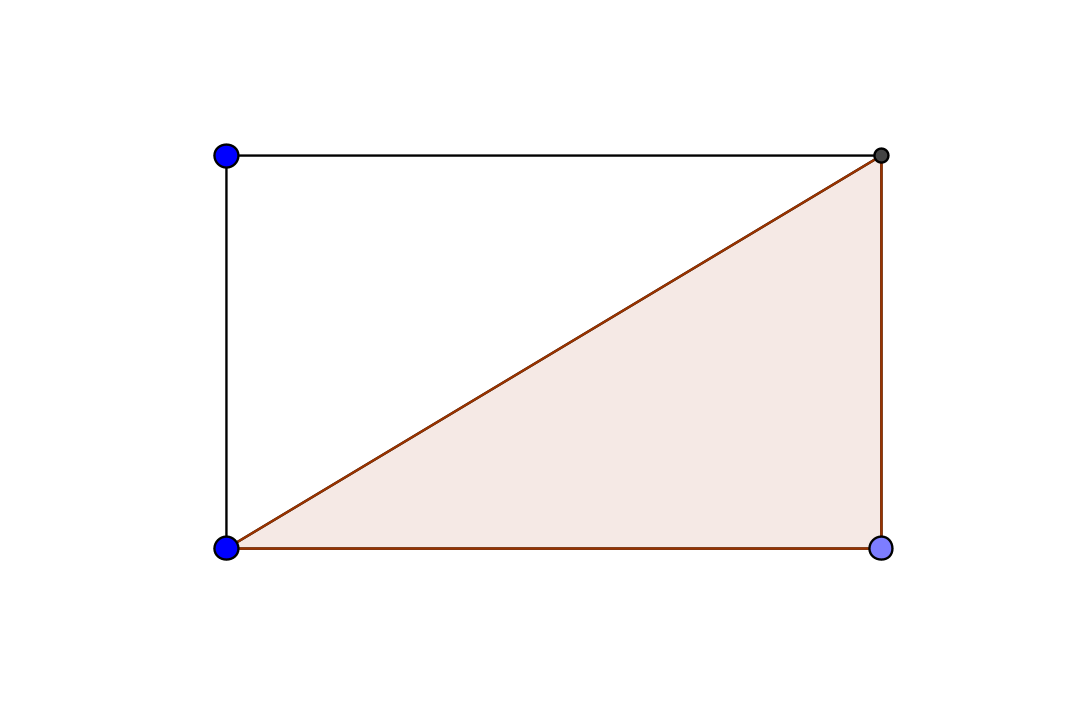
\includegraphics[width=1.2\linewidth]{0a}
\caption{1a)}
\endminipage\hfill
\minipage{.32\textwidth}
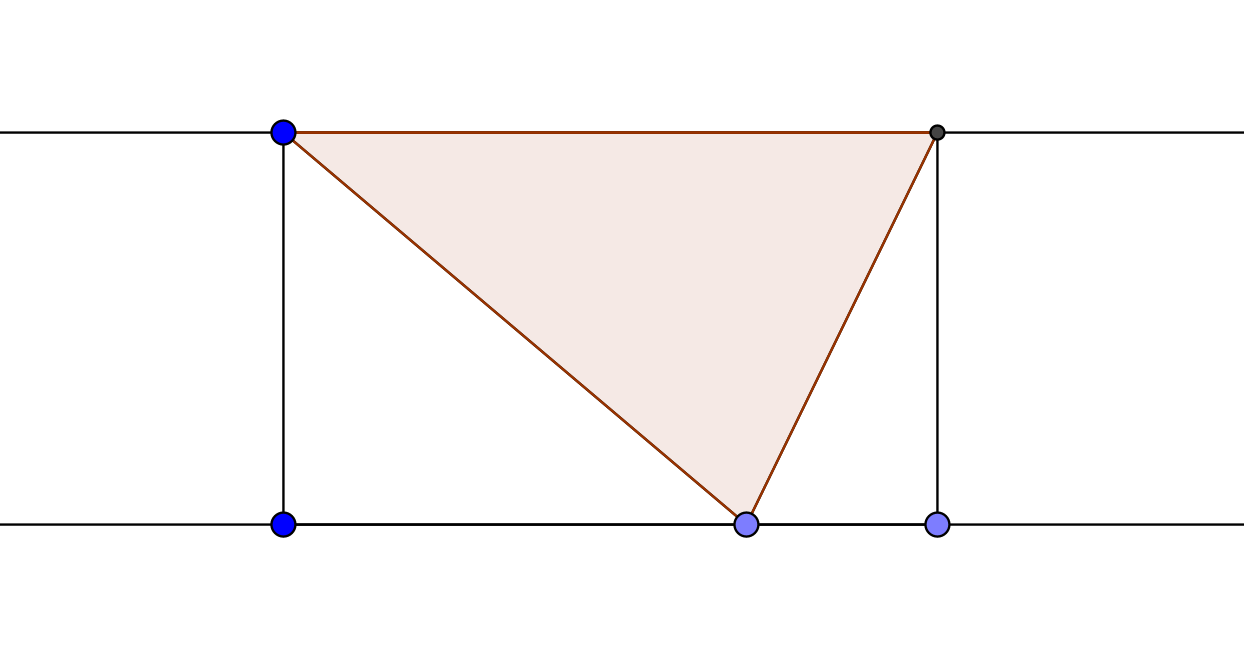
\includegraphics[width=1.2\linewidth]{0c}
\caption{1a)}
\endminipage\hfill
\minipage{.32\textwidth}
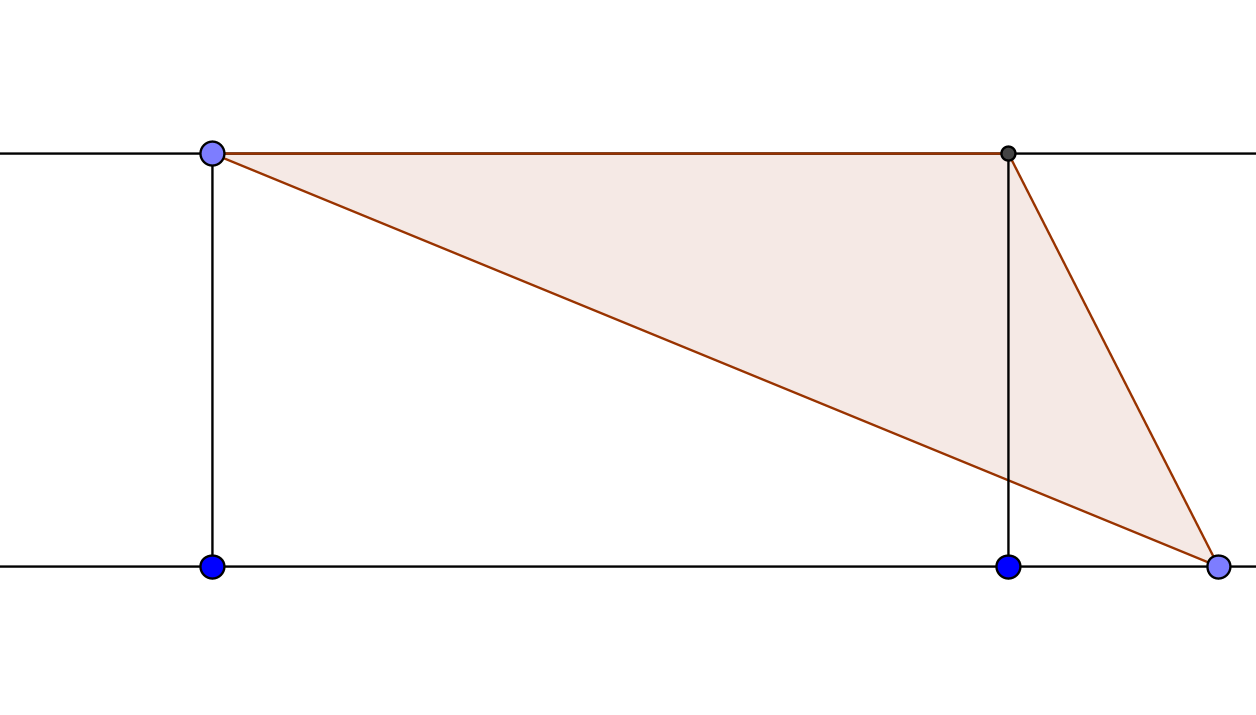
\includegraphics[width=1.2\linewidth]{0b}
\caption{1c)}
\endminipage
\end{figure}

\begin{figure}[h]
\minipage{.32\textwidth}
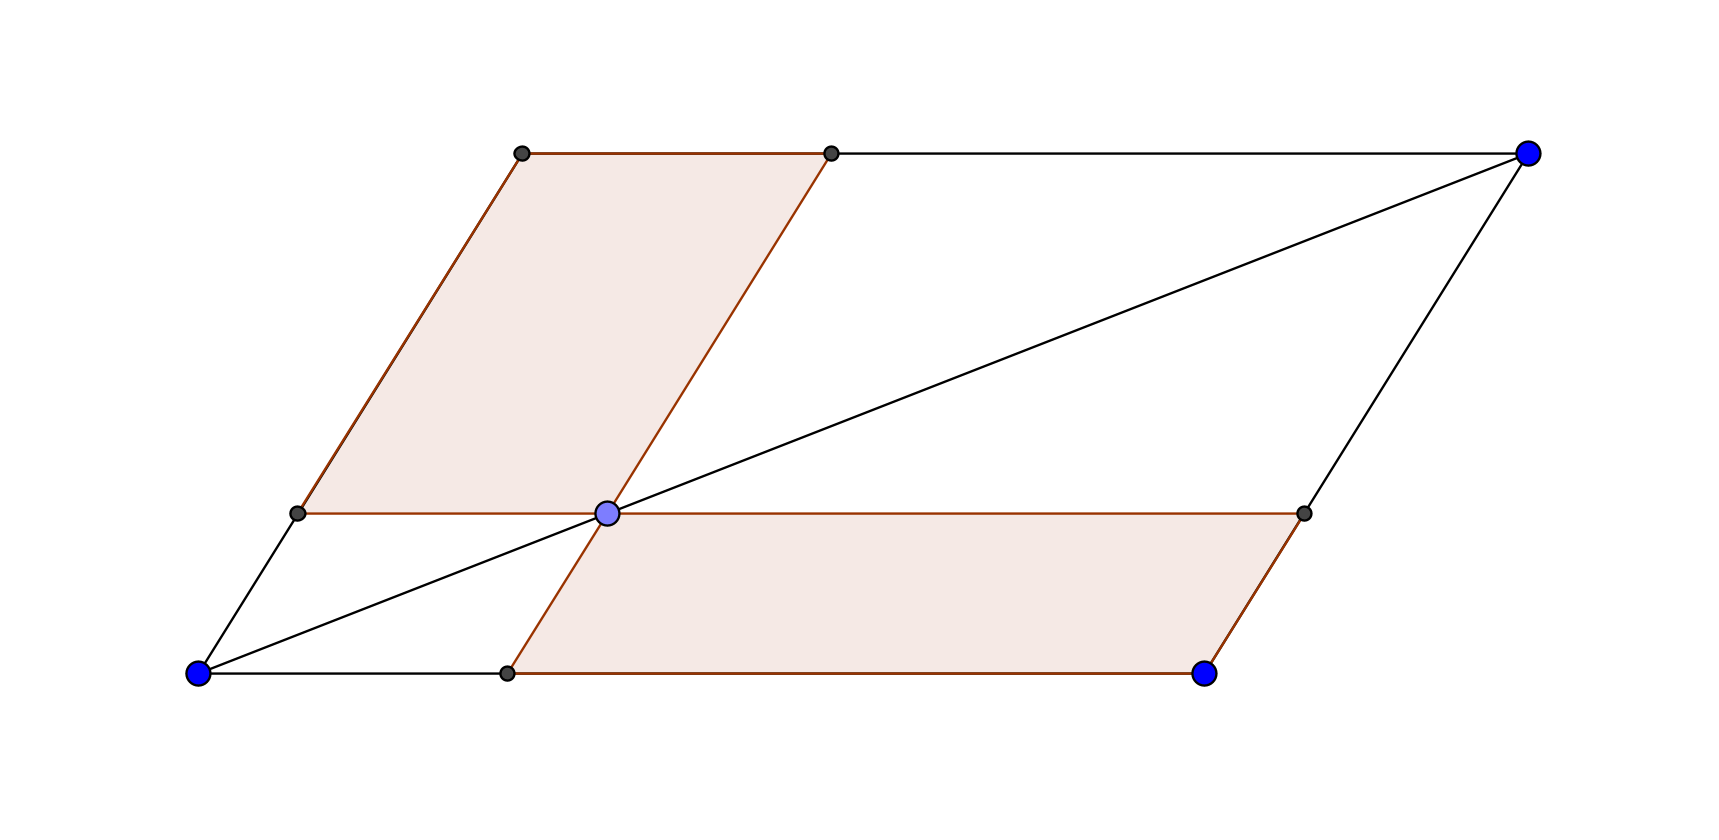
\includegraphics[width=1.2\linewidth]{1}
\caption{2)}
\endminipage\hfill
\minipage{.32\textwidth}
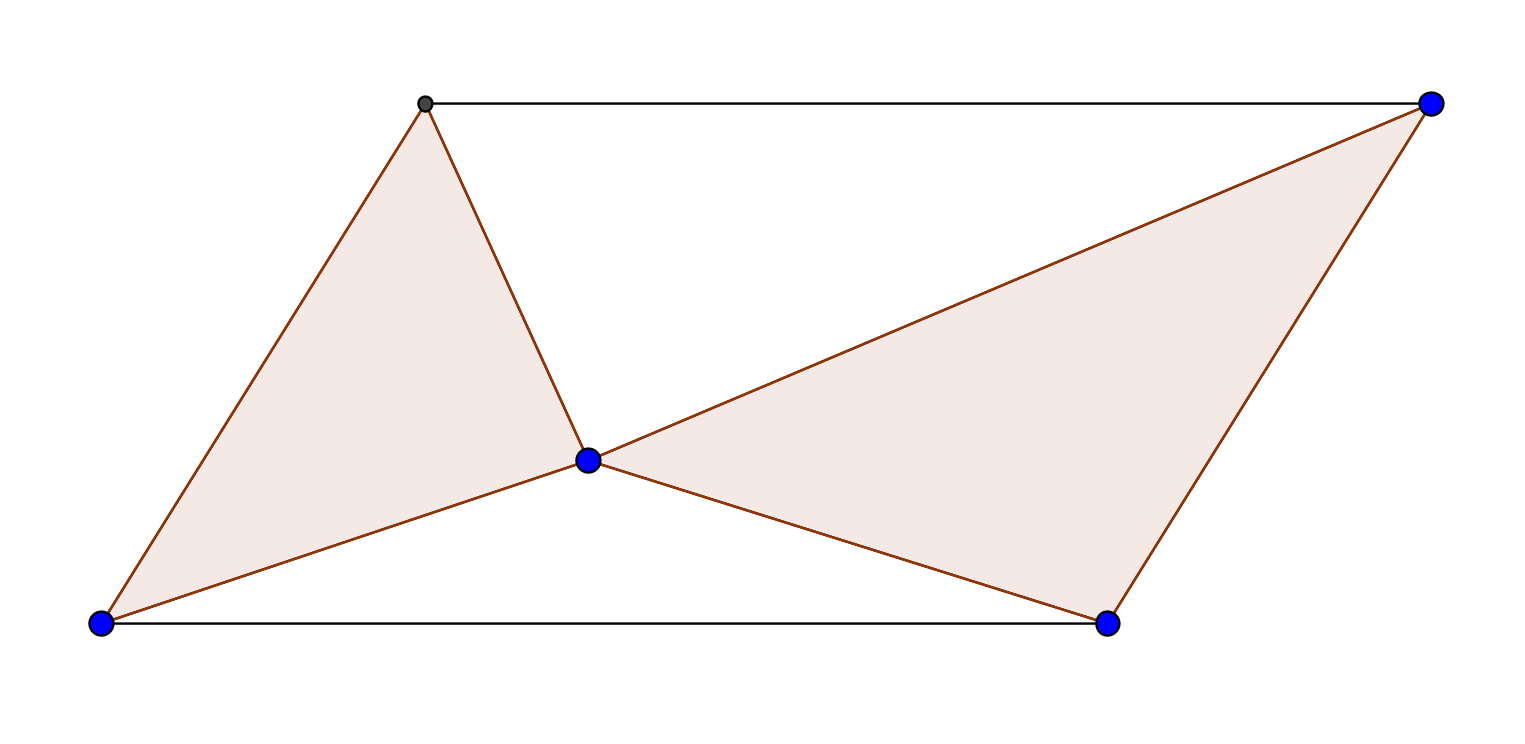
\includegraphics[width=1.2\linewidth]{2b}
\caption{3)}
\endminipage\hfill
\minipage{.32\textwidth}
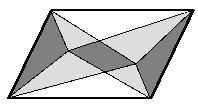
\includegraphics[width=1.2\linewidth]{2d}
\caption{5a)}
\endminipage
\end{figure}

\begin{figure}[h]
\minipage{.32\textwidth}
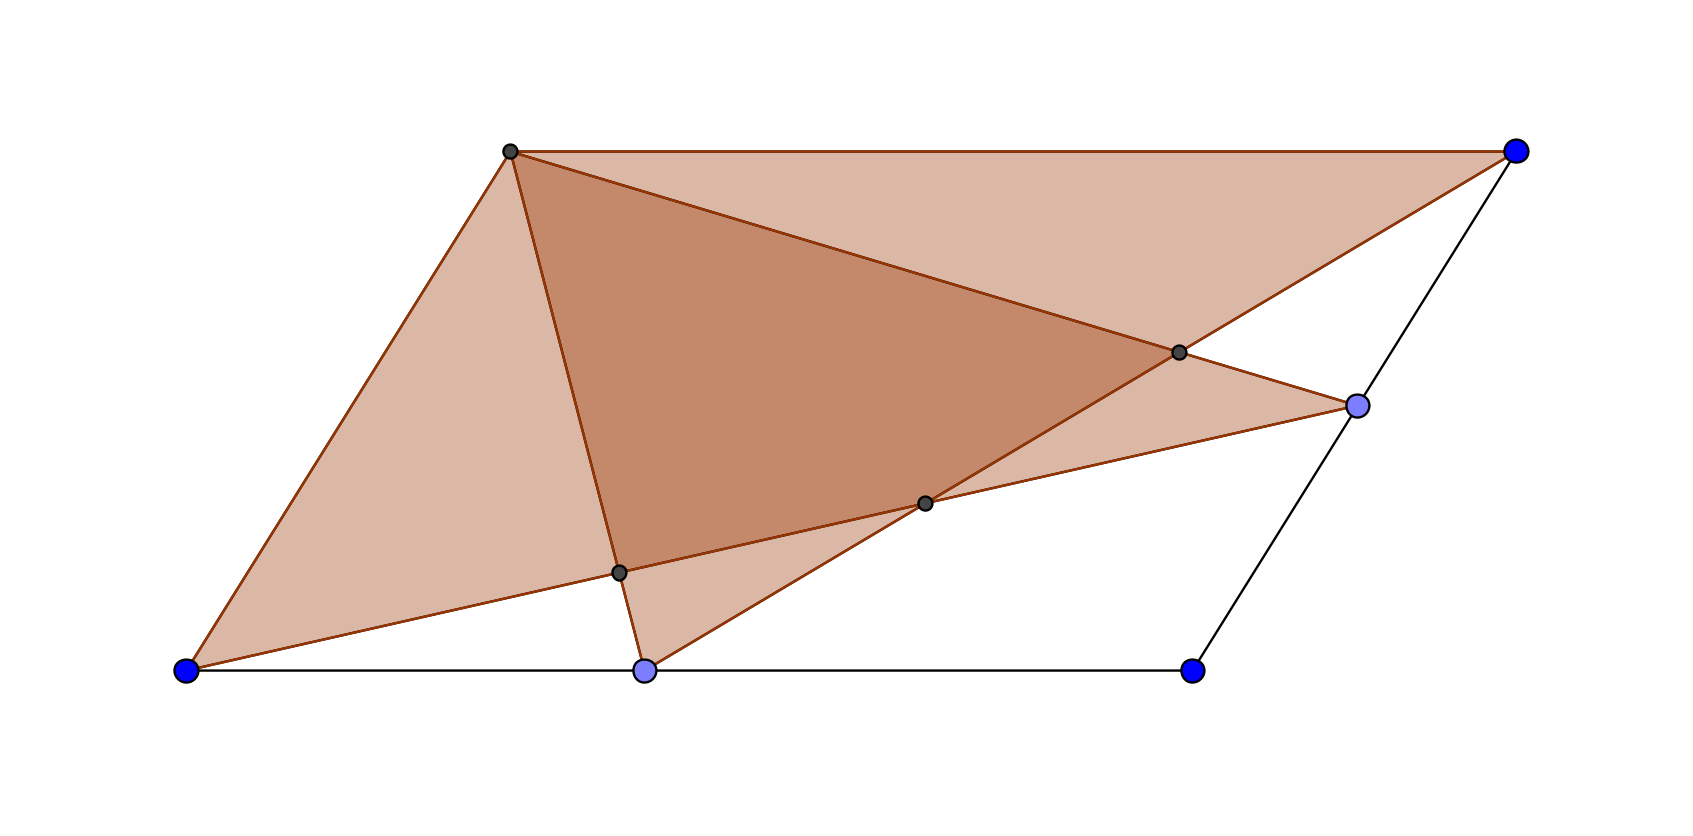
\includegraphics[width=1.2\linewidth]{2c}
\caption{5b)}
\endminipage\hfill
\minipage{.32\textwidth}
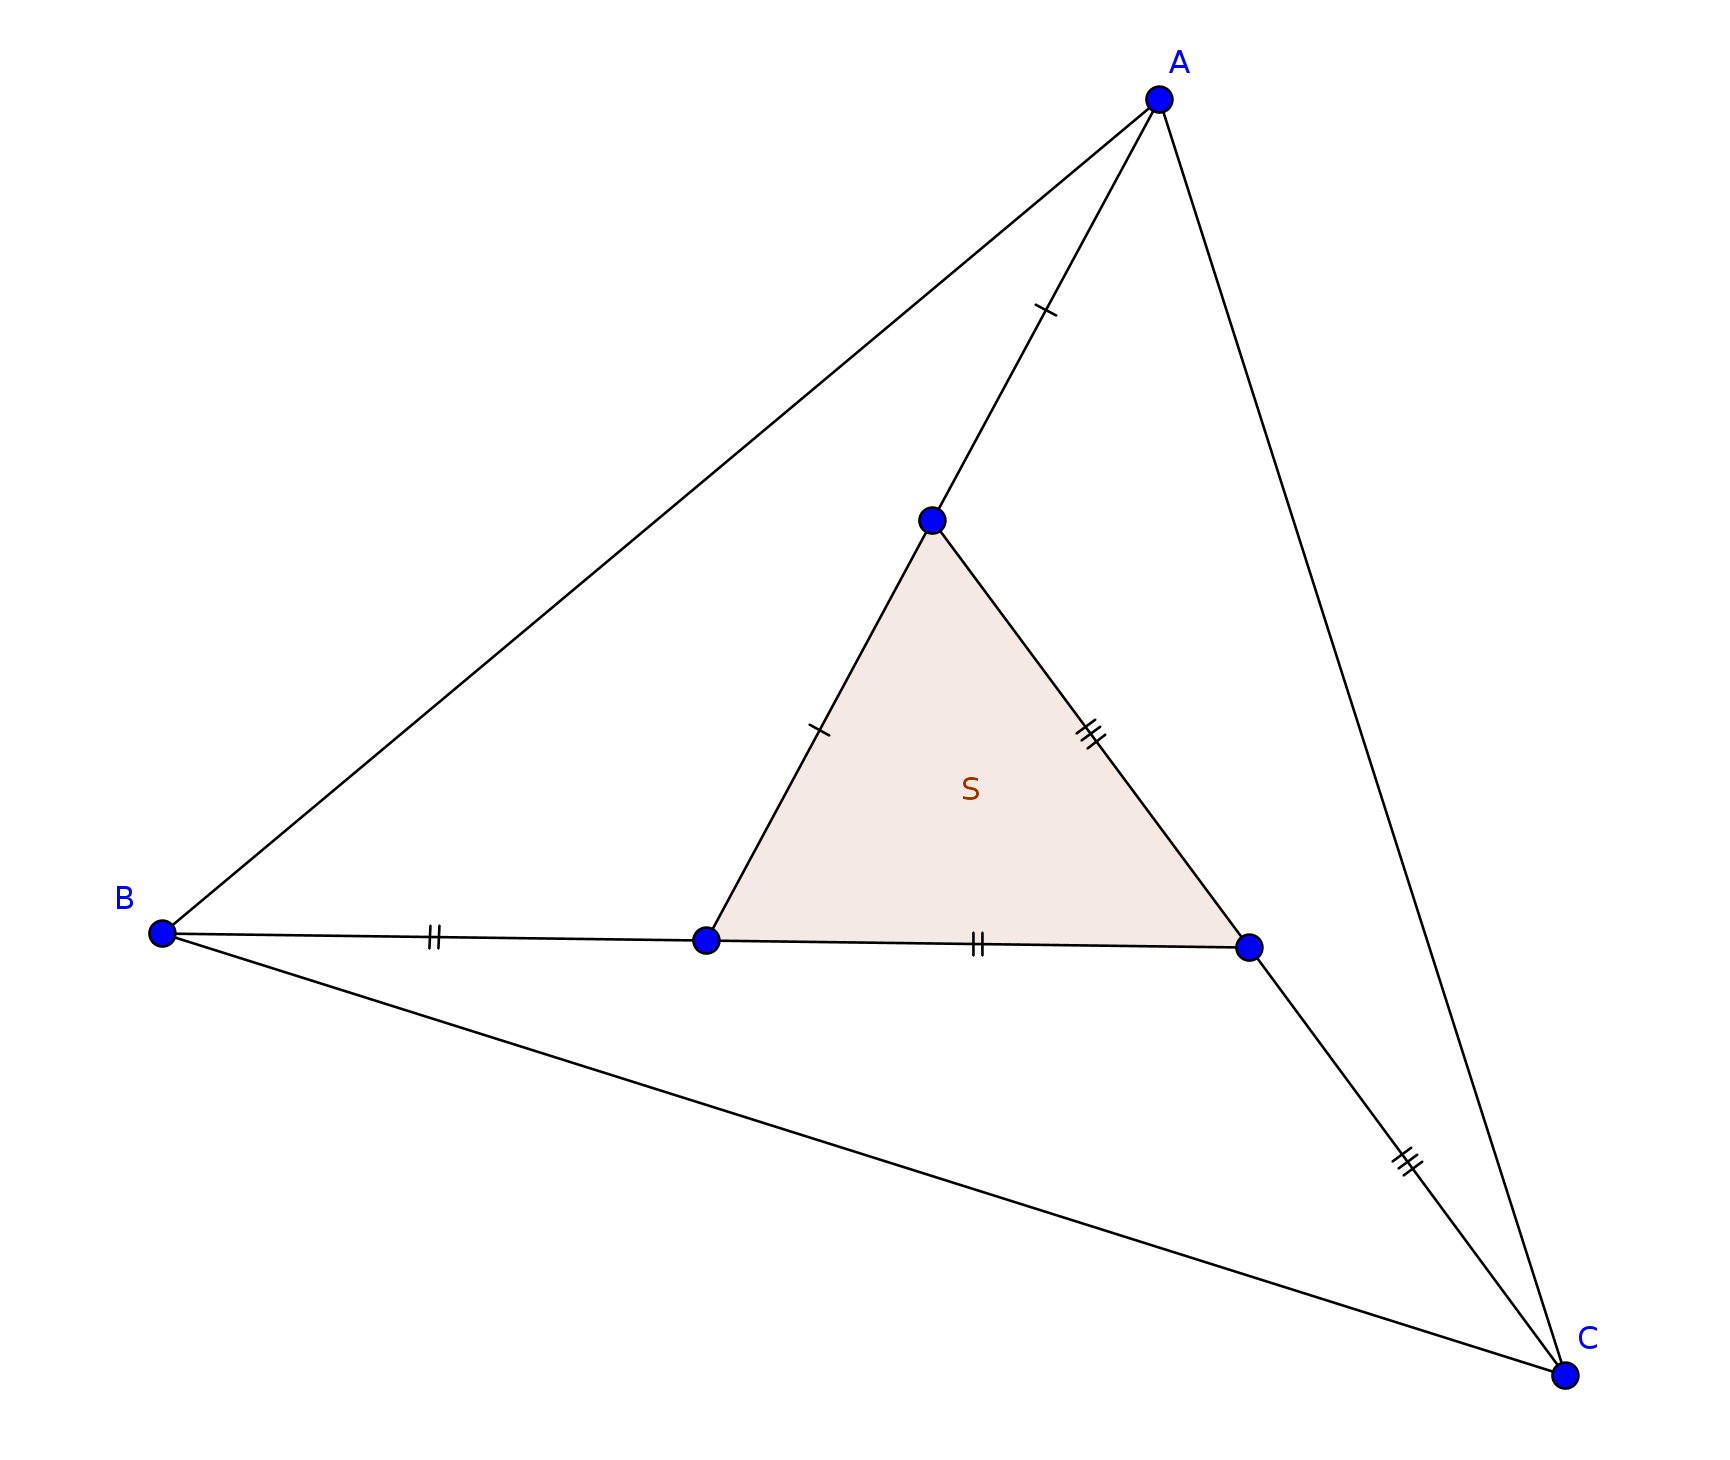
\includegraphics[width=1.2\linewidth]{7a}
\caption{7a)}
\endminipage\hfill
\minipage{.32\textwidth}
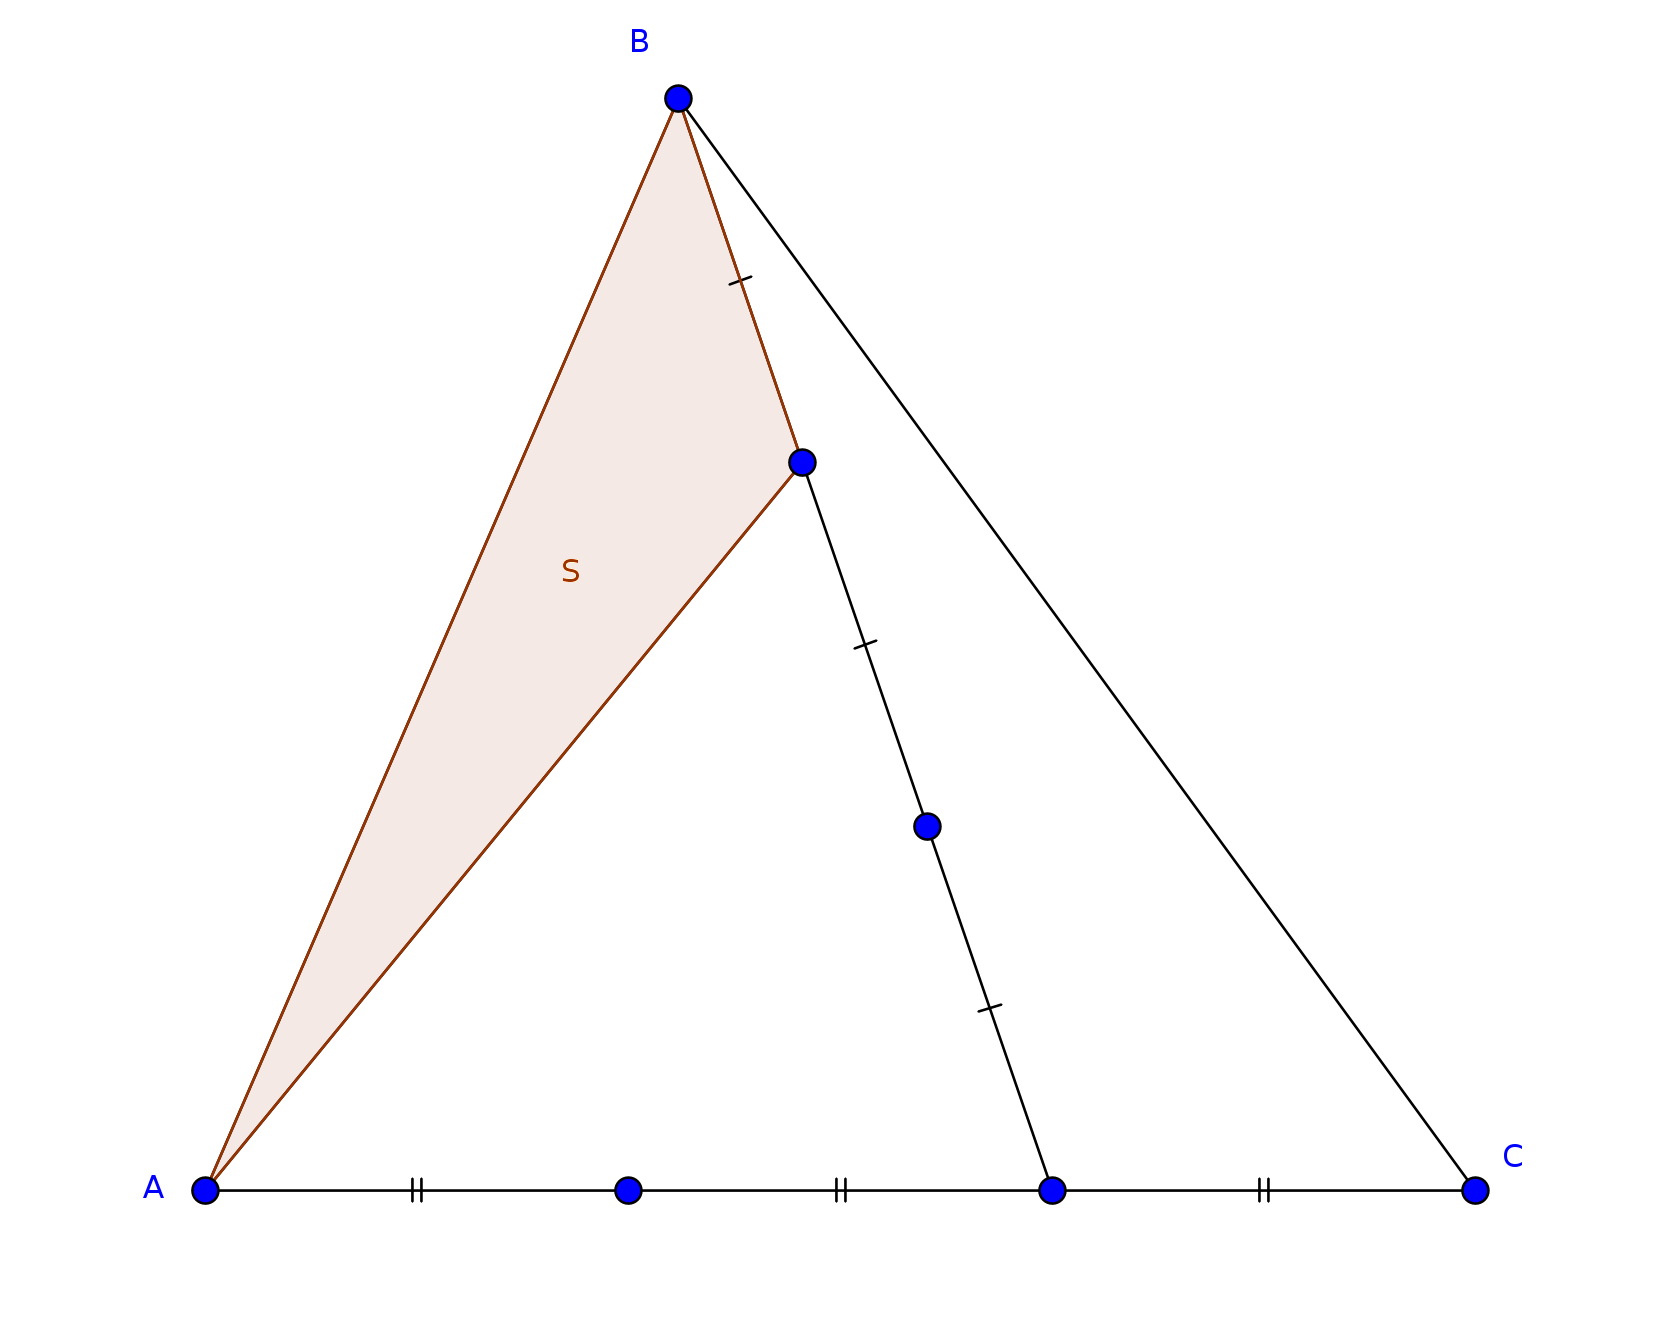
\includegraphics[width=1.2\linewidth]{7b}
\caption{7b)}
\endminipage
\end{figure}

\begin{figure}[!h]
\minipage{.32\textwidth}
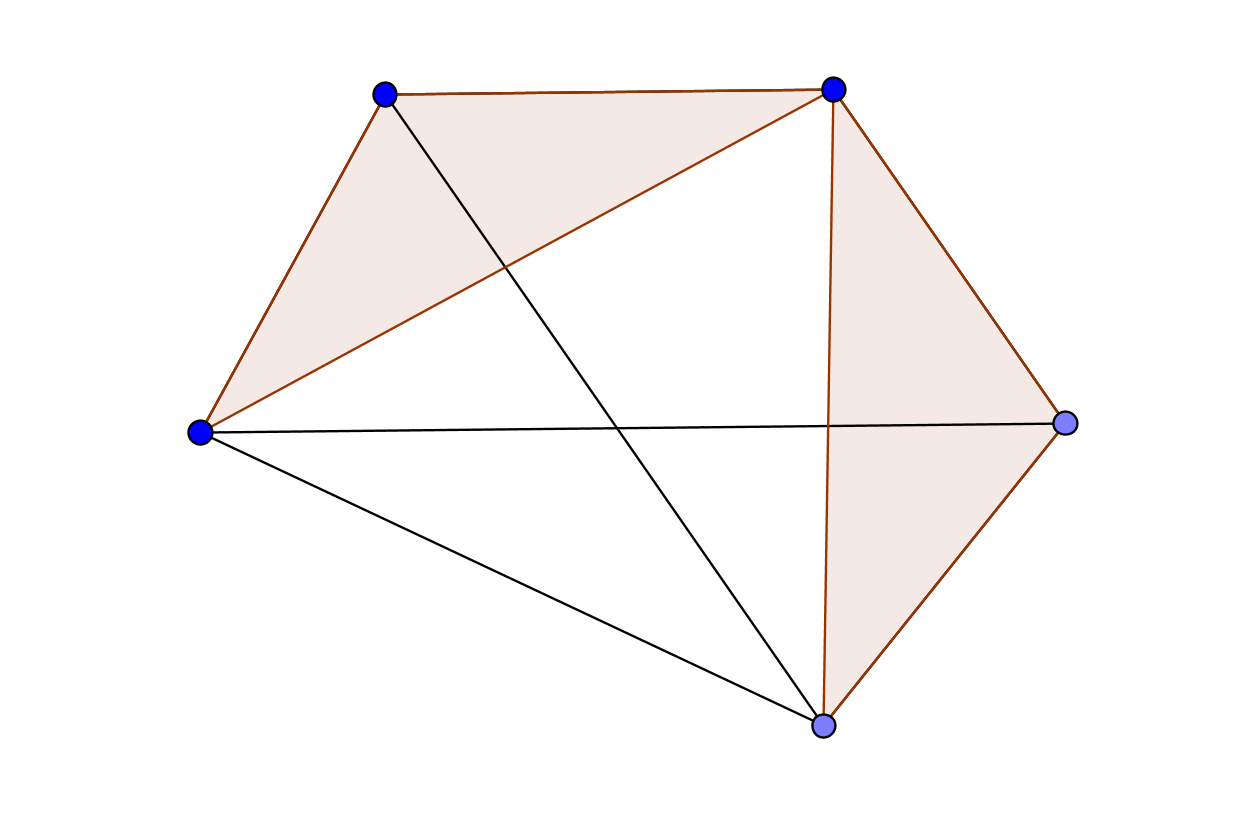
\includegraphics[width=1.2\linewidth]{5}
\caption{8)}
\endminipage\hfill
\minipage{.32\textwidth}
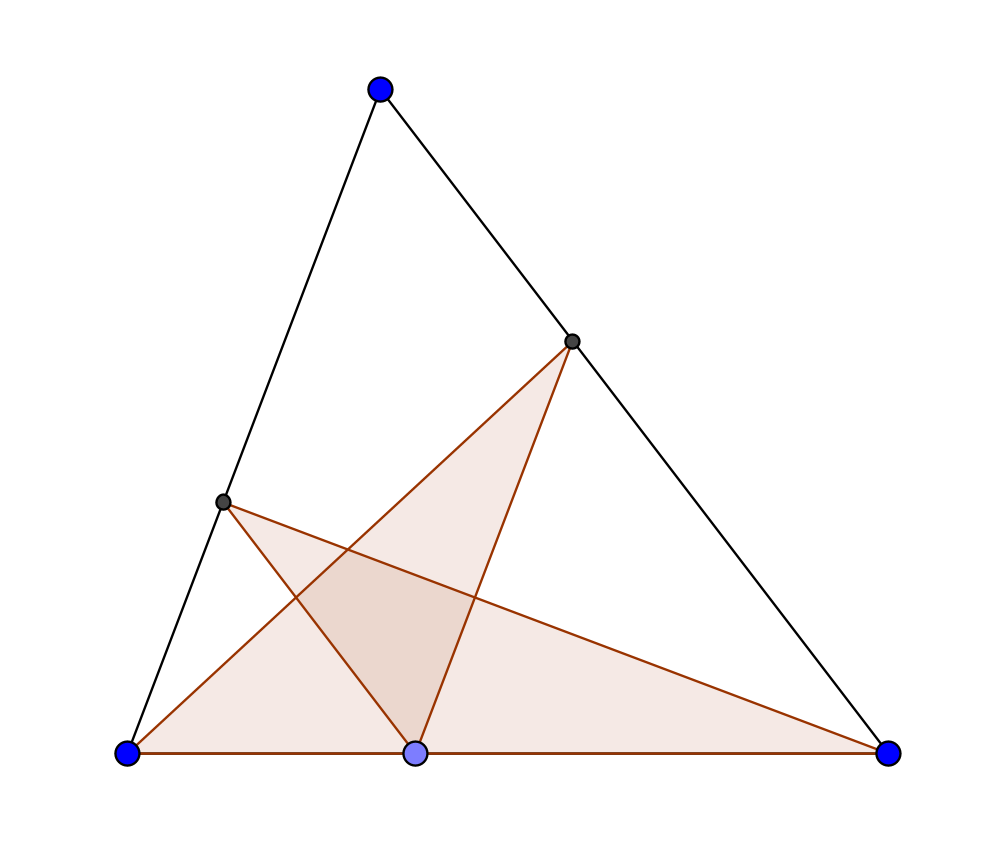
\includegraphics[width=1.2\linewidth]{6}
\caption{9)}
\endminipage\hfill
\minipage{.32\textwidth}
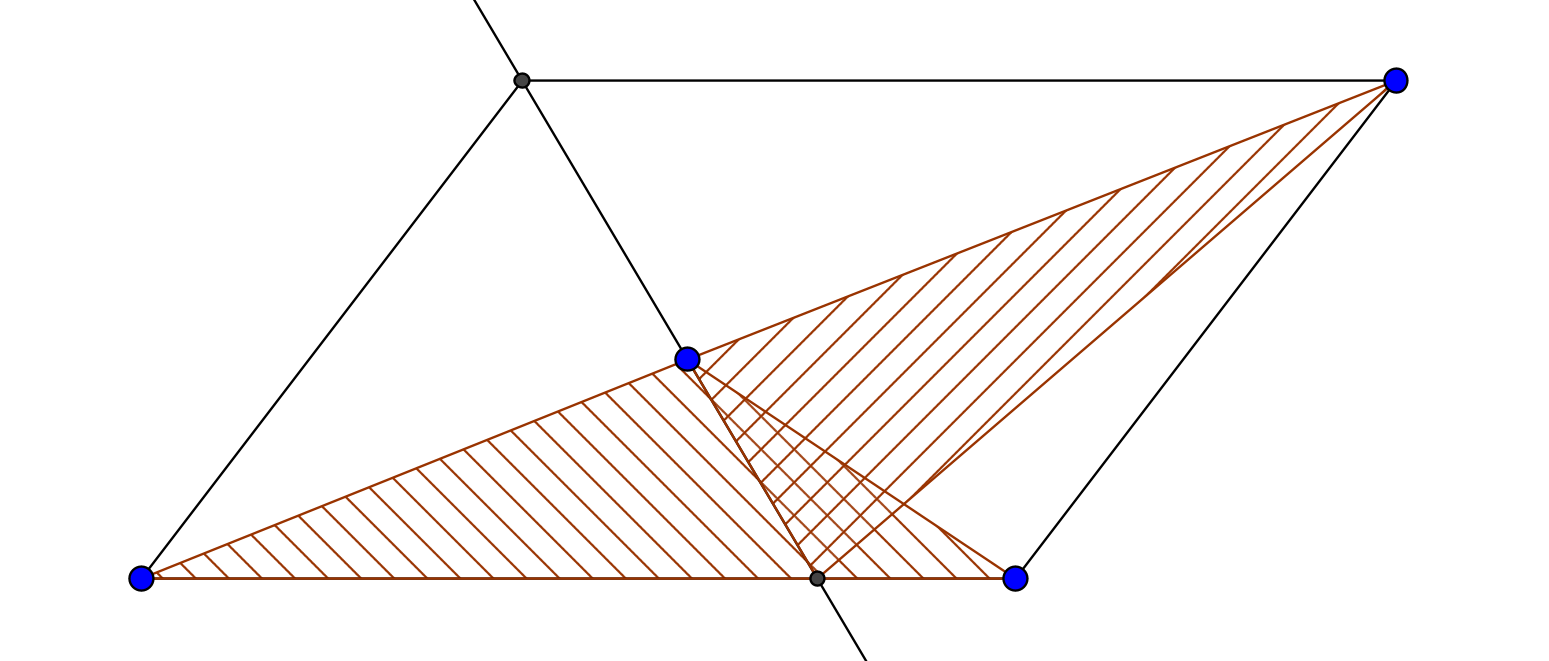
\includegraphics[width=1.2\linewidth]{3}
\caption{10)}
\endminipage
\end{figure}

\begin{figure}[!h]
\minipage{.32\textwidth}
% \includegraphics[width=\linewidth]{5d}
% \caption{7)}
\endminipage\hfill
\minipage{.32\textwidth}
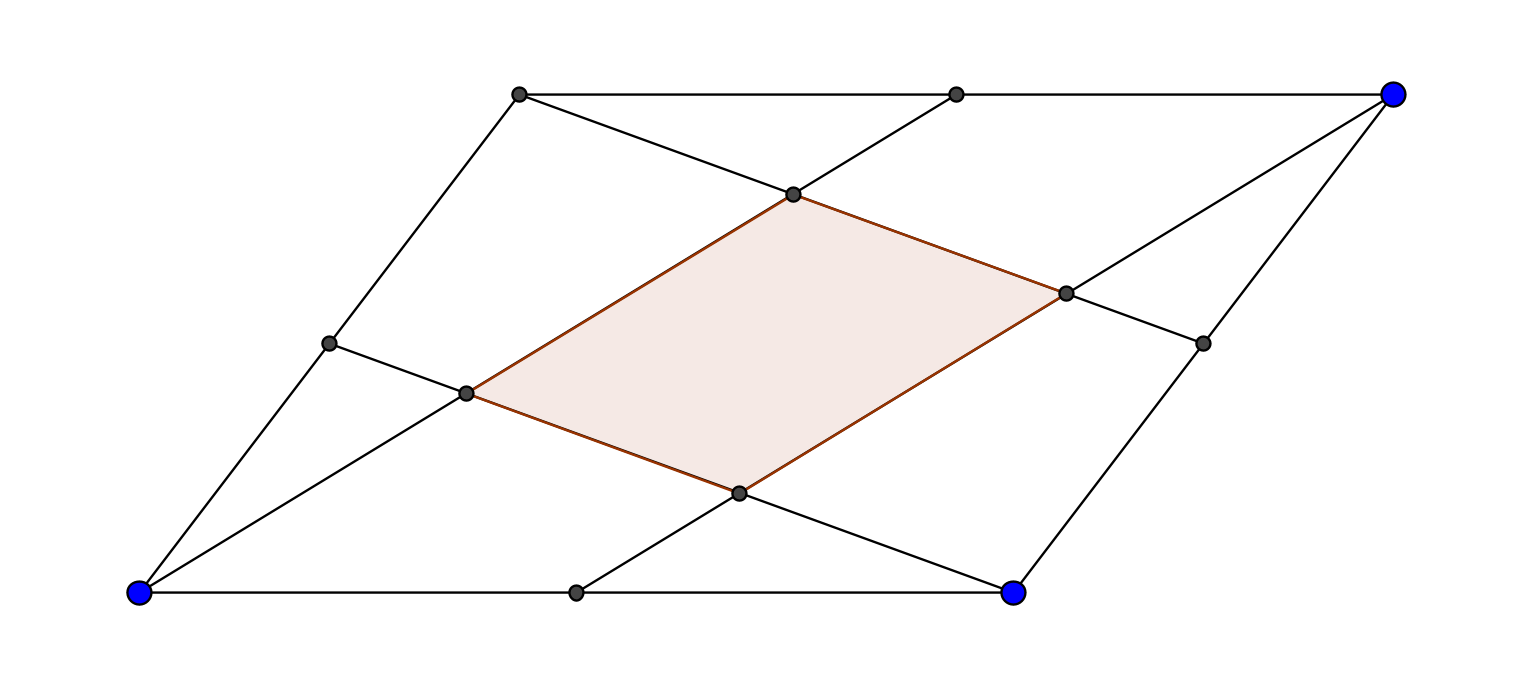
\includegraphics[width=1.2\linewidth]{4}
\caption{12)}
\endminipage\hfill
\minipage{.32\textwidth}
% 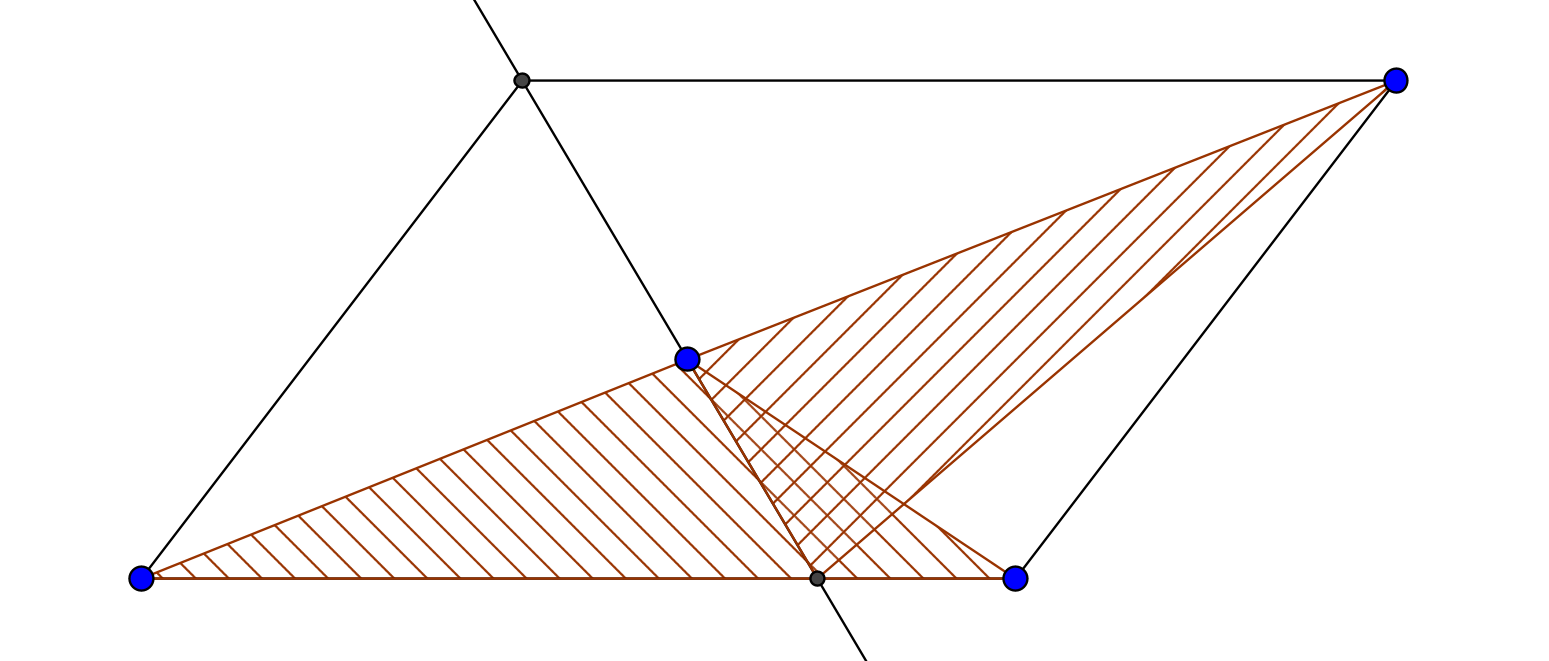
\includegraphics[width=\linewidth]{3}
% \caption{10)}
\endminipage
\end{figure}

\quad\newpage